% 电介质
% 电偶极子|位移极化|取向极化|电偶极矩|无极分子|有极分子
\pentry{电偶极子\upref{eleDpl}}

首先来了解一下何为电介质.
\begin{definition}{电介质}
\textbf{电介质(dielectric)}是电阻率很大、导电能力很差的物质,其主要特征在于它的原子或分子中的电子与原子核的结合力很强,电子处于束缚状态.当电介质处在电场中时,在电介质中,不论是原子中的电子、还是分子中的离子或是晶体点阵上的带电粒子,在电场的作用下都会在原子大小的范刚内移动,当达到静电平衡时,在电介质表面层或在体内会出现极化电荷,这个现象称作电介质的\textbf{极化(polarization)}.
\end{definition}
下面就研究电场与电介质间的相互作用,从而说明电介质的一些性质.

\subsection{电介质的电结构}

电介质中每个分子都由正、负电荷组成,是一个复杂的带电系统一般来说,正、负电荷在分子中都不集中在一点,但在考虑这些电荷在离分子较远处所产生的电场时,或是考虑一个分子受外电场作用时,可以认为分子中的全部正电荷可用一等效正电荷来代替,全部负电荷用一等效负电荷来代替等效正、负电荷在分子中所处的位置,分别称为该分子的\textbf{正负电荷“中心”}.

按照电介质分子内部的电结构不同,可以把电介质分为两大类:有极分子和无极分子.有一类电介质,如水蒸气($\rm H_2O$)、氯化氢($\rm HCl$)、一氧化碳($\rm CO$) 、氨($\rm NH_3$)等,分子内正、负电荷中心不相重合,这类分子称为\textbf{有极分子(polar molecules)}.设有极分子的正电荷中心和负电荷中心之间的距离为$l$,分子中全部正电荷或负电荷的总电荷量为$q$,则有极分子的等效电偶极矩$\mathbf p=q\mathbf l$.整块电介质可以看成是无数个电偶极子的聚集体,虽然每一个分子的等效电偶极矩不为零,但由于分子的无规则热运动,各个分子的电偶极矩的方向是杂乱无章地排列的,所以不论从电介质的整体来看,还是从电介质中的某一小体积(其中包含有大量的分子)来看,其中各个分子电偶极矩的矢量和$\sum \mathbf p$平均说来等于零,电介质是呈电中性的.
\begin{figure}[ht]
\centering
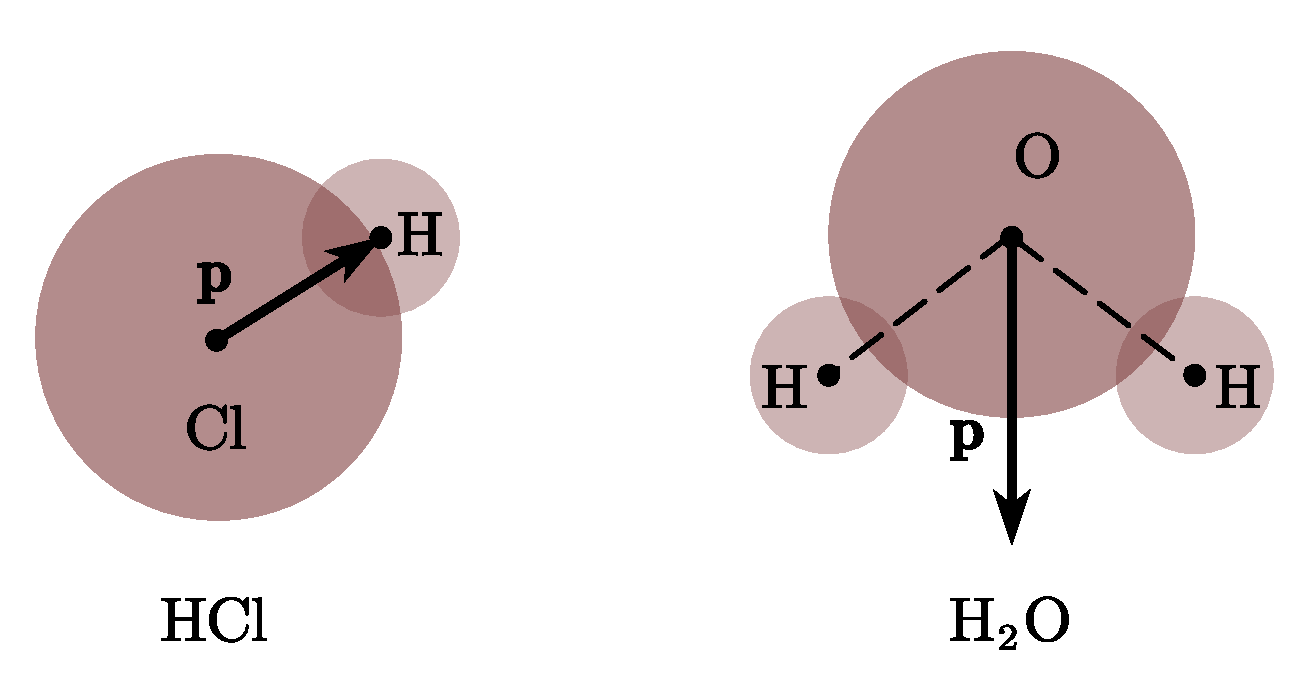
\includegraphics[width=8.5cm]{./figures/Dielec_1.pdf}
\caption{有极分子的电偶极矩示例} \label{Dielec_fig1}
\end{figure}
另有一类电介质,如氢($\rm H_2$)、氦($\rm He$)、氮($\rm N_2$)、甲烷($\rm CH_4$) 等,它们的正、负电荷的中心重合在一起,它的等效电偶极矩等于零,凡属于这种类型的分子叫做\textbf{无极分子(nonpolar molecules)}.由于每个分子的等效电偶极矩$\mathbf p=0$,电介质整体也是呈电中性的.

基于有极分子和无极分子的电结构不同,它们在外电场中所受到的作用也不相同,下面将分别讨论.

\subsection{电介质的极化}

\subsubsection{无极分子电介质的位移极化}

当无极分子电介质处在外电场中时,在电场力作用下分子中的正、负电荷中心将发生相对位移,形成一个电偶极子,它们的等效电偶极矩$\mathbf p$的方向都沿着电场的方向\autoref{Dielec_fig2} (b) 所示.在电介质内部,由于相邻电偶极子的正负电荷相互靠近,如果电介质是均匀的,则在它内部仍然保持电中性,但是在电介质的两个和外电场强度$\mathbf E_0$相垂直的表面层里(厚度为分子等效电偶极矩的轴长$l$)将分别出现正电荷和负电荷.这些电荷不能离开电介质,也不能在电介质中自由移动,我们称之为\textbf{极化电荷(polarized charge)}.把在电场作用下能移动一宏观距离的电荷统称为\textbf{自由电荷(free charge)}.这种在外电场作用下,在电介质中出现极化电荷的现象叫做\textbf{电介质的极化}.分子的电偶极矩$\mathbf p $的大小与电场强度成正比,外电场越强,每个分子的正、负电荷中心之间的相对位移越大,分子的电偶极矩也越大,电介质两表面上出现的极化电荷也越多,被极化的程度越高.当外电场撤去后,正、负电荷的中心又重合在一起,见$\mathbf p=0$,\autoref{Dielec_fig2} (a).电介质表面上的极化电荷也随之消失.由于无极分子的极化来自正、负电荷中心的相对位移,所以常叫做\textbf{位移极化(displacement polarization)}.
\begin{figure}[ht]
\centering
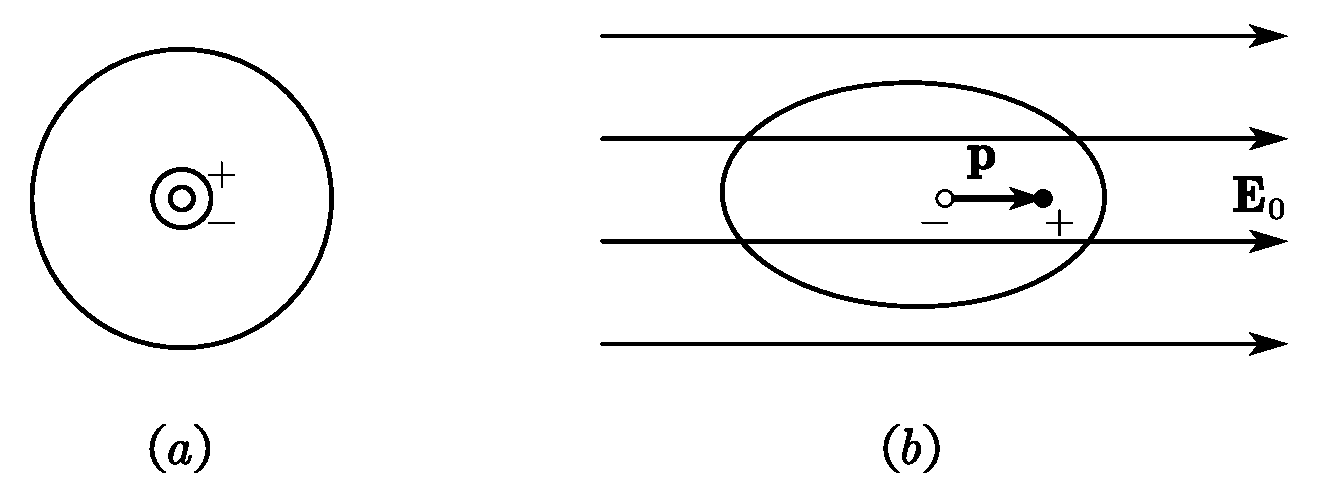
\includegraphics[width=10cm]{./figures/Dielec_2.pdf}
\caption{无极分子极化示意图} \label{Dielec_fig2}
\end{figure}

\subsubsection{有极分子电介质的取向极化}

对于有极分子电介质来说,每个分子本来就等效为一个电偶极子,它在外电场的作用下,将受到力矩的作用,使分子的电偶极矩$\mathbf p$转向电场的方向,如\autoref{Dielec_fig3} (b)所示.这样,宏观上看,在电介质与外电场垂直的两表面上也会出现极化电荷,如\autoref{Dielec_fig3} (c)所示.当外电场撤去后,由于分子无规热运动和分子间的相互碰撞都会破坏分子偶极矩沿电场方向的取向排列,使之回到沿各个方向的均匀分布(\autoref{Dielec_fig3} (a)),表面的极化电荷也随之消失.可见,有极分子电介质的极化程度取决于外电场的强弱和电介质的温度,外电场越强且温度越低,分子电偶极矩沿电场取向排列的概率也越大.有极分子的极化就是等效电偶极子转向外电场的方向,所以叫做\textbf{取向极化(orientation polarization)}.一般说来,分子在取向极化的同时还会产生位移极化,但是,对有极分子电介质来说,在静电场作用下,取向极化的效应比位移极化的效应强得多,因而其主要的极化机理是取向极化.
\begin{figure}[ht]
\centering
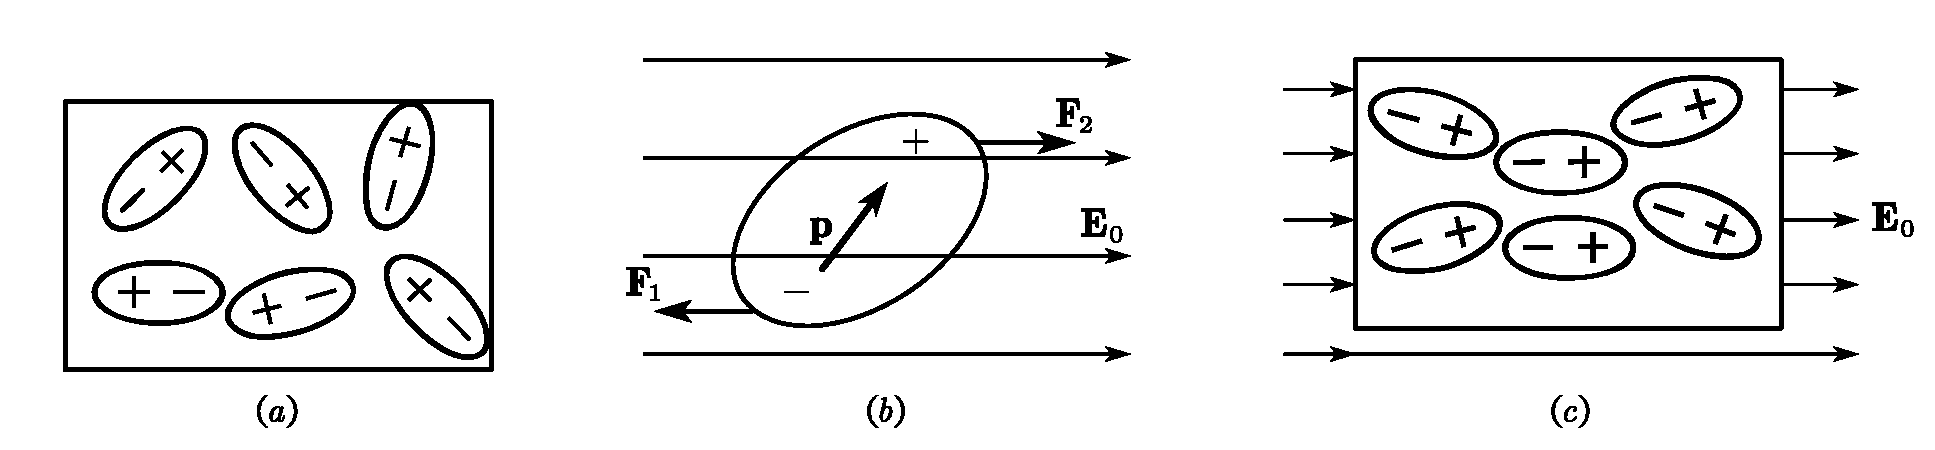
\includegraphics[width=14.25cm]{./figures/Dielec_3.pdf}
\caption{有极分子的极化示意图} \label{Dielec_fig3}
\end{figure}

当前广为应用的家用微波炉,就是介质分子(水分子)在高频电场中反复极化的一个实际应用!水分子作为一个有极分子,其电偶极子在电场力矩的作用下,要转向与外电场方向一致的排列.如果电场方向交替变化,水分子的电偶极矩$\mathbf p$也要跟随电场方向反复转动,在这个过程中水分子作高频振动,引起快速摩擦而产生热量.当微波频率为$2450\rm  MHz$时,水分子能极大地吸收微波的电磁能量,达到加热、煮熟食物的目的.微波在金属面上反射,却很容易穿透空气、玻璃、塑料等物质,且极大地被食物中的水、油、糖所吸收.
